\begin{event}{WP6 Workshop: Knowledge representation in mathematical software and databases}{wp6-0}{St Andrews (UK), 2016-01-25 to 2016-06-27}{JU,SA,PS,UV,UW,ZH}{12}{}

  \textbf{Main goals.} Semiannual \ODK project meeting joined with a
  WP6 ``Data/Knowledge/Software bases'' kickoff workshop dedicated to
  the exploration of how mathematical knowledge could be better
  represented and exploited within systems and for communicating
  between systems.


\textbf{ODK implication.} St Andrews hosted this event which was
organized by Paris Sud (project meeting) and Jacobs Uni (WP6 workshop).

\textbf{Event summary.} Tuesday morning was dedicated to \ODK's
semiannual
\href{http://opendreamkit.org/meetings/2016-01-25-DKS/SteeringCommittee/minutes/}
{steering committee meeting}, including progress reports from all
sites. A couple additional \ODK participants joined physically or
remotely for this meeting.

The rest of the week was dedicated to Work Package 6 activities. To
bootstrap the discussions, we started with a presentation by Michael
Kohlhase of his ideas for a Knowledge First strategy, followed by
presentations of how knowledge is represented in various components of
\ODK (FindStat: Viviane Pons, LMFDB: Paul-Olivier Dehaye, GAP: Markus
Pfeiffer, SageMath: Nicolas M. Thiéry), in preparation for
\longdelivref{dksbases}{design}. There was also a brief presentation
of a proof-of-concept Knowledge-aware Sage-GAP interface developed the
week before at the GAP/Sage Days. Current practices where discussed as
well: commonalities in ``dumping math data on the web'' process
(FindStat, LMFDB,…). Then came a tutorial presentation of MMT to
explore how knowledge representation in MMT could serve as a generic
knowledge backbone for integrating the various systems.  After these
warm up activities, we moved on to brainstorms and joint code sprints,
developing proof-of-concepts formalizations of the knowledge in the
various components and exploring applications: detecting bugs and
inconsistencies in code and data, generating more complete
documentation, supporting generic handle interfaces, \ldots

A fine grained report of the activities is available
\href{http://opendreamkit.org/meetings/2016-01-25-DKS/report/}{here}.

\textbf{Results and impact.} The Math-in-the-Middle approach was born
at this workshop. This led to a joint paper at the CICM
conference~\cite{DehKohKon:iop16} and kicked off and fueled much of
the activity on WP6 since then, in particular around
\longtaskref{dksbases}{data-design}, \delivref{dksbases}{design},
\delivref{dksbases}{dkstheories}, and
\delivref{component-architecture}{semantic-interface-sage-gap}.

\begin{figure}[ht]
  \caption*{WP6 Workshop: Knowledge representation in mathematical software and databases}
  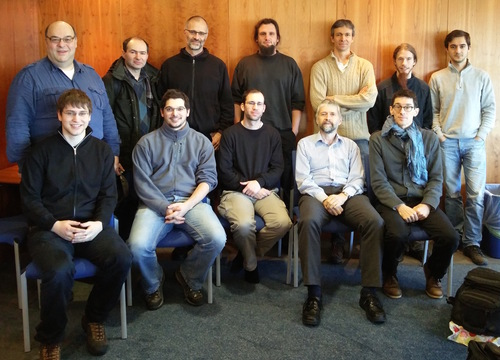
\includegraphics[scale=0.5]{pictures/2016-01-25-DKS-group-picture.jpg}
  \end{figure}
\end{event}
